\chapter{Introduction}
\label{chap:One}
\section{Motivation}
LEGOs have been one of the most popular games in the world since our childhood to this day. Every person, whether a child or an adult, want to express their creativity and show their skills. This is achieved by designing buildings, houses and many architectural objects using LEGOs and trying different designs. In this project, we aim to create an app where anyone can design and create 3D models (mostly influenced by the Islamic art) using LEGOs to be converted to 3d mesh models that could be 3D printed as well as creating a video play-back of this creation process.\par

\section{Problem Statement}
The aim of this thesis is to investigate the use of Generative Adversarial Networks (GANs) to create realistic synthetic ultrasound images of breast tissue for the detection and diagnosis of breast cancer. The problem lies in the challenge of generating high-quality synthetic images that accurately reflect the complexity of breast tissue while avoiding the generation of misleading features. The proposed research will focus on developing a GAN-based framework that can effectively capture the essential features of breast tissue in ultrasound images and generate synthetic images that are indistinguishable from real ultrasound images. The research will evaluate the performance of the proposed framework by comparing the generated images to real ultrasound images and assessing the accuracy of breast cancer diagnosis using the synthetic images. The results of this research will contribute to the development of a reliable and accurate tool for breast cancer diagnosis and treatment.
 \vspace{1cm}


\section{Objectives}
The objectives of this work are:
\begin{itemize}
\item A literature review summarizing previous research on ultrasound imaging for breast cancer detection, as well as prior work on GANs for image generation.
\item A dataset of real ultrasound images of breast tissue, along with corresponding annotations indicating the presence or absence of cancer.
\item A GAN model trained on the dataset that is capable of generating synthetic ultrasound images of breast tissue with or without cancerous lesions.
\item Evaluation of the synthetic images generated by the GAN, including measures of image quality and similarity to real ultrasound images.
\item A tool or platform for healthcare professionals to access and use the synthetic images to improve their diagnostic accuracy and efficiency.
\item A technical report detailing the methodology and results of the project, including any limitations or potential areas for future work.
\item Presentation materials such as slides or posters for sharing the project.
\item A journal paper summarizing the project and its findings.
\item Open-source code and documentation for the GAN model and associated tools, enabling other researchers to replicate or build upon the work.
\end{itemize}
 \section{Project Plan and Block Diagram }
 \begin{figure}[H]
    \centering
    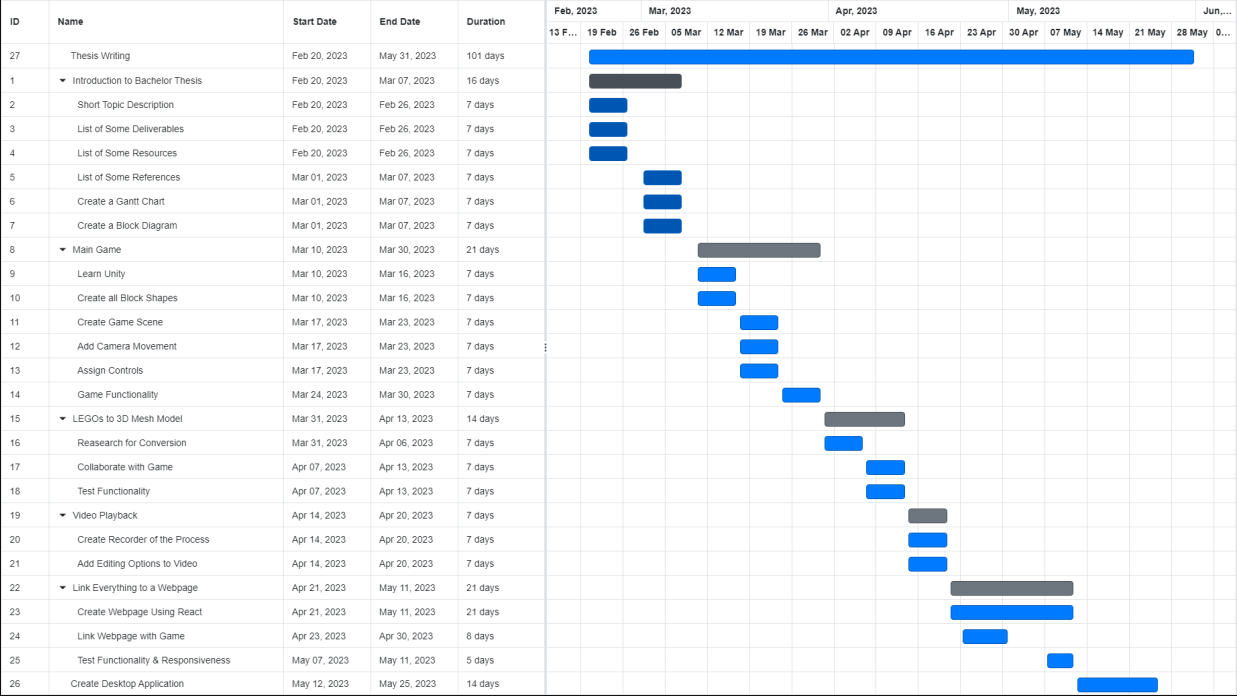
\includegraphics[width = 15 cm]{Project Plan.png}
    \caption{Project Plan}
    \label{fig:Project Plan ScreenShot}
\end{figure}
\begin{figure}[H]
    \centering
    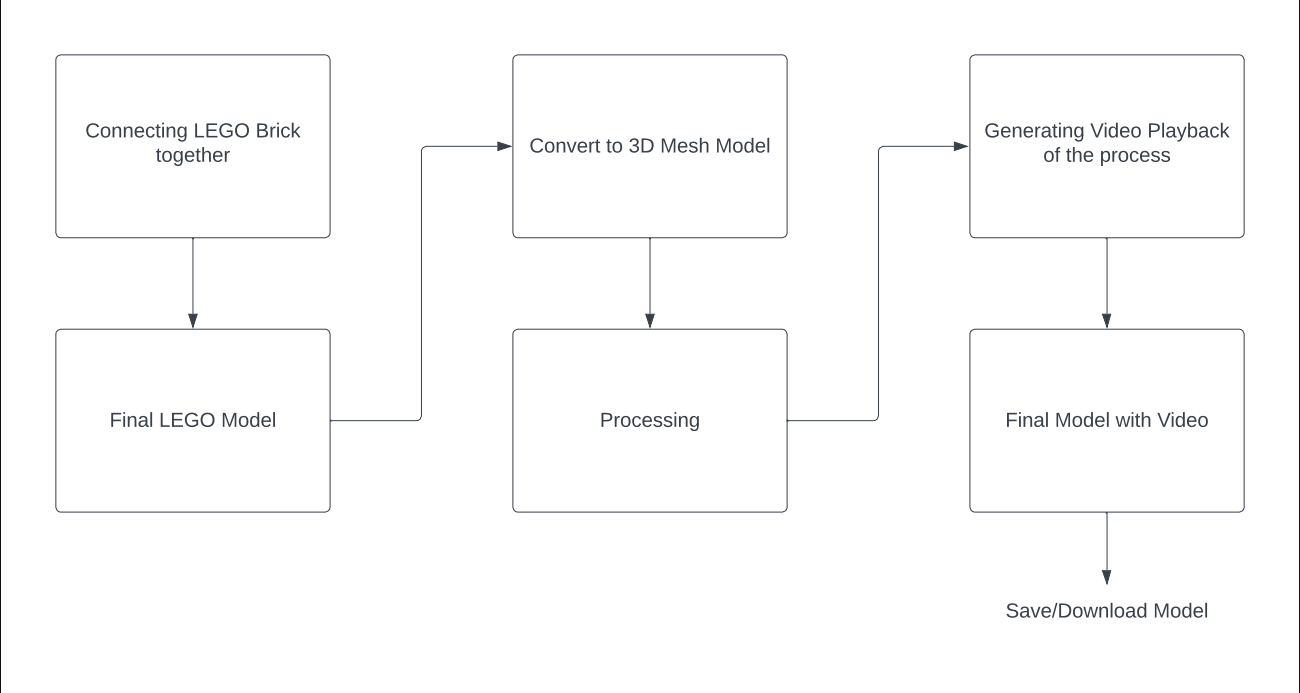
\includegraphics[width = 15 cm]{Block Diagram.png}
    \caption{Block Diagram }
    \label{fig:Block Diagram ScreenShot}
\end{figure}
\section{Thesis Outline}
In this thesis we will ..... In \ref{chap:One} we discuss the..... The second chapter \ref{sec:ConceptsOverview} is the explanation of .....
In \ref{sec:LiteratureReview} is also a summary of previous work done ..... 
Chapter \ref{chap:Three} is how the project was developed, 


\begin{itemize}
\item \textbf{Concept Overview:} A brief explanation of all technologies used throughout the paper.
\item \textbf{Literature Review:} A compilation of all previous work done in the past regarding the implemented project or any of the technologies used.
\item \textbf{Methodology:} Workflow overview on how the project was implemented and how the environment developed could be replicated.
\item \textbf{Results:} The section is split into to parts the first part compares between datasets tried and the second part is the results received from the project.
\item \textbf{Conclusion:} A brief discussion of what was achieved in this paper, and the future work that could be done to excel the results and further development.
\end{itemize}

